\section{Topic Tree}

\subsection{Home Page}

From the homepage, a user (both students and academics) can get to the topic tree from the sidebar.\\

\begin{figure}[h!]
    \centering
    
\includegraphics[scale=0.4]{topic-tree-dashboard}
    \caption{Topic Tree Link in Dashboard}
\end{figure}

This allows quick access to the topic tree so students can easily view which topics they must complete next and academics can also easily edit topics and upload content.\\

\subsection{Views}

The main feature of the topic tree is the graph view. Here the user can view the topic groups, topics and how each topic is related to each other (through prerequisites). On first load, the topic groups are shown with arrows to indicate the prerequisites. In the below screenshot, there is a topic in Programming Fundamentals that is a prerequisite for a topic in C++ Programming i.e. a student must complete the topic in Programming Fundamentals before they can start topics in C++ Programming.\\

\begin{figure}[h!]
    \centering
    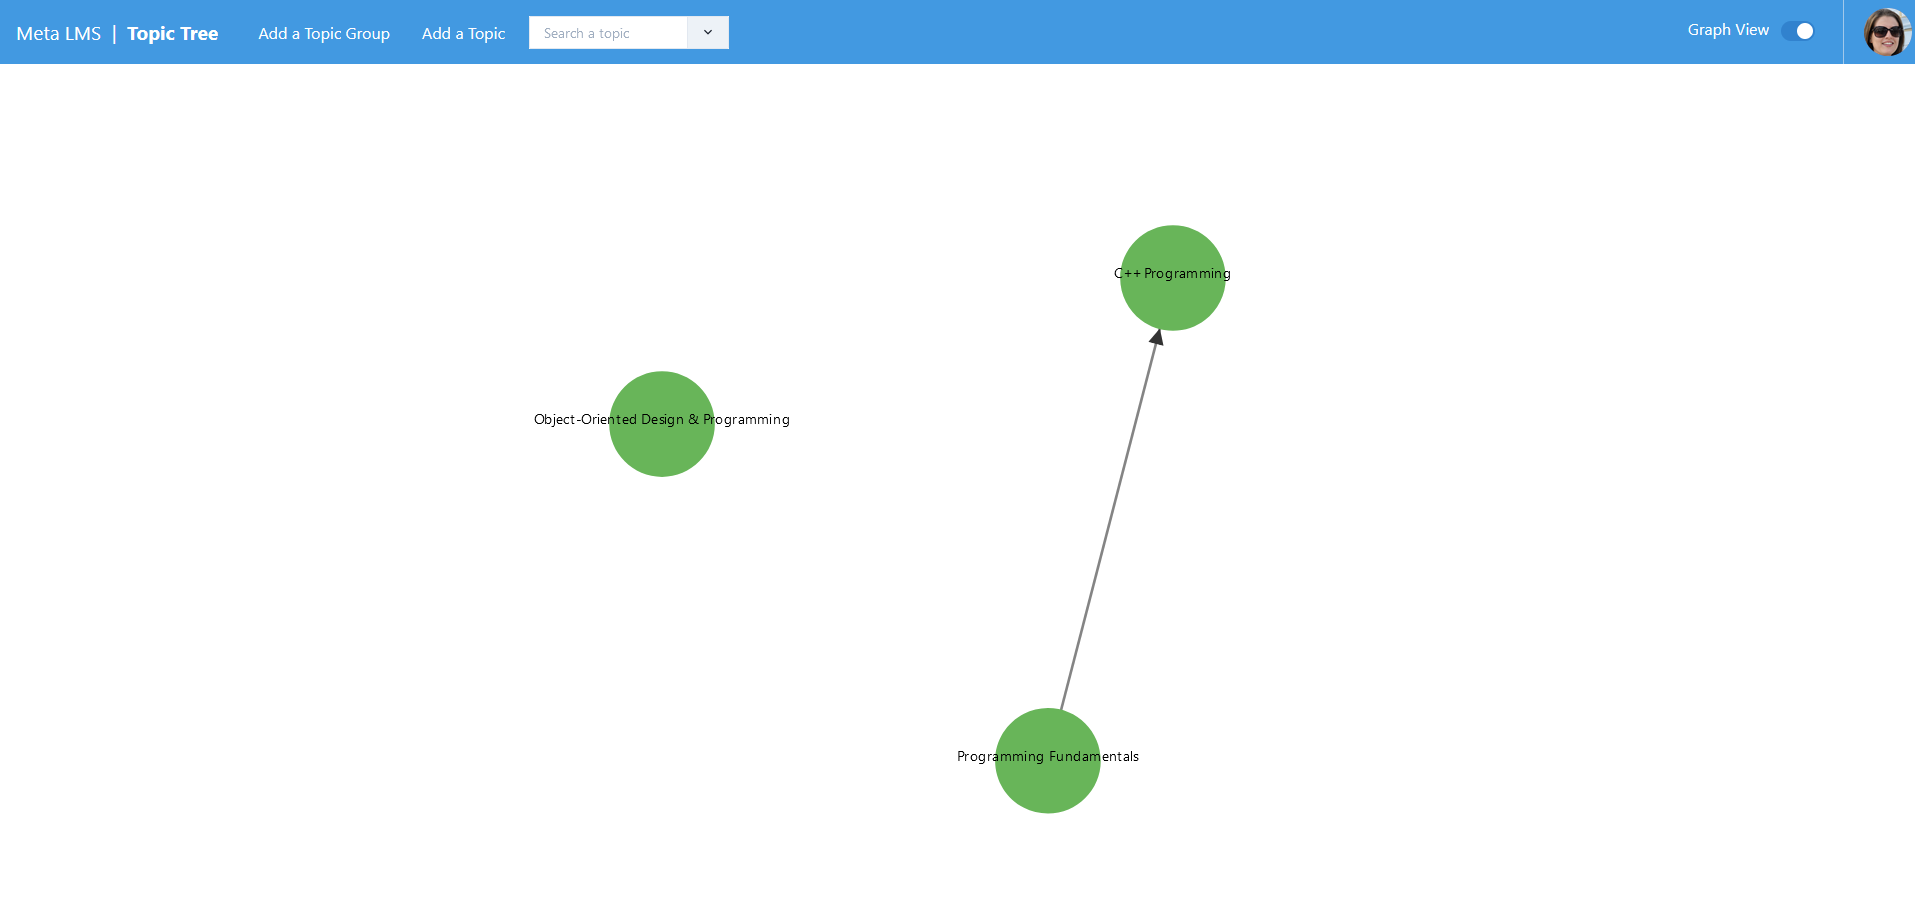
\includegraphics[scale=0.4]{topic-tree-graph-view-actual}
    \caption{Topic Tree Graph View}
\end{figure}

A topic group is marked as green, and when clicked it expands into the individual topics as shown below. \\

\begin{figure}[h!]
    \centering
    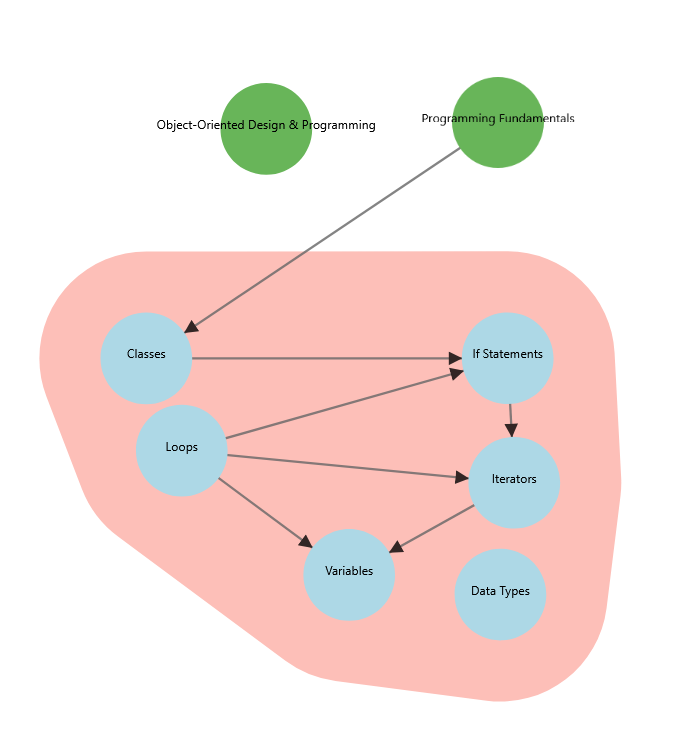
\includegraphics[scale=0.4]{topic-tree-expanded}
    \caption{Topic Tree Expanded}
\end{figure}

A hull around the topics is drawn to indicate that they are part of the same topic group, as in the above example the topics are part of C++ Programming.\\

\begin{figure}[h!]
    \centering
    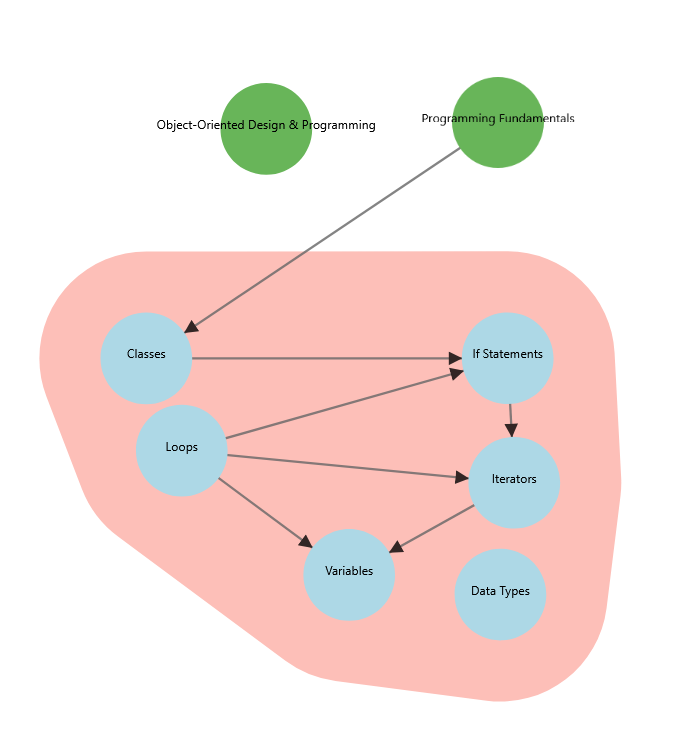
\includegraphics[scale=0.4]{topic-tree-hull}
    \caption{Topic Tree - Hull}
\end{figure}

The graph can be zoomed in, and you can drag topics out to make topics to be more visible. Some users may want to view the topics in a list instead of a graph.\\

\begin{figure}[h!]
    \centering
    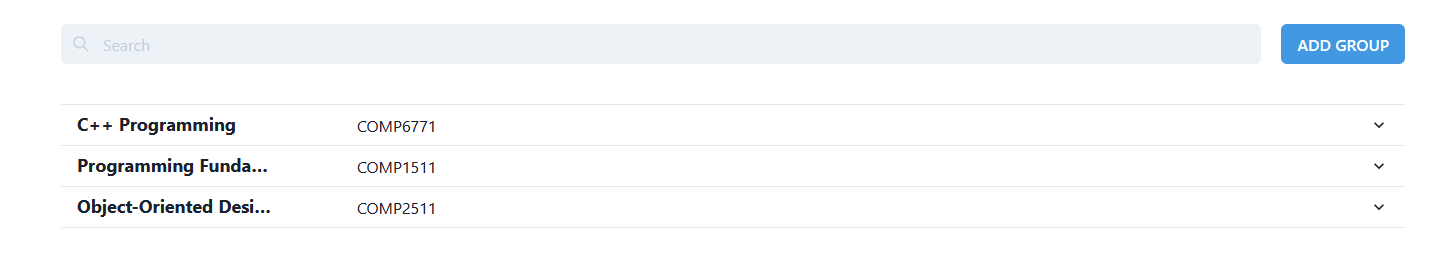
\includegraphics[scale=0.4]{topic-tree-list-actual}
    \caption{Topic Tree - List View}
\end{figure}

A list of the various topic groups is viewable, and when a topic group is clicked, the topics that are in the topic group expands as shown below.\\

\begin{figure}[h!]
    \centering
    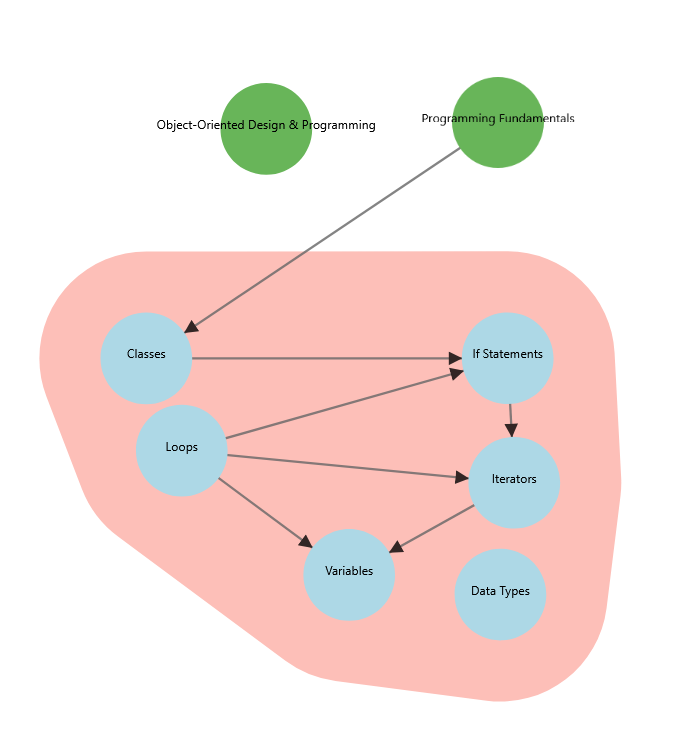
\includegraphics[scale=0.4]{topic-tree-expanded}
    \caption{Topic Tree - List View Expanded}
\end{figure}

\subsection{Resources}

When a topic is clicked on the graph view or the list view, the user can then view the prerequisites of that topic, tags for search optimisation, and any files associated with the topic.

\begin{figure}[h!]
    \centering
    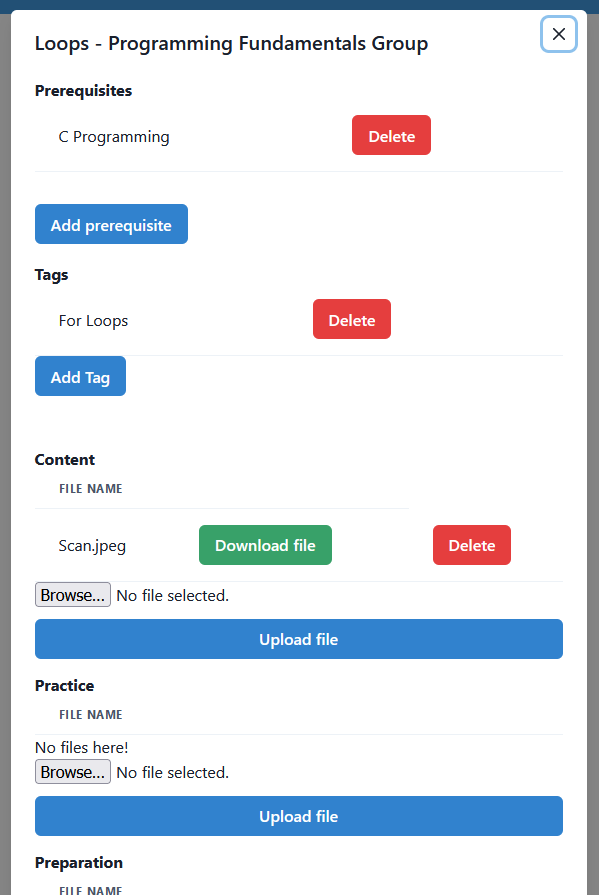
\includegraphics[scale=0.4]{topic-tree-view-resource}
    \caption{Topic Tree - View Resource}
\end{figure}

There are four file sections: Content, Practice, Preparation and Assessments. This is so it is adaptable to most learning models. Academics can upload any file they would like to a topic, and it will be viewable for all to view. In the future, permissions will be implemented to restrict access to certain resources. Third party integration with services such as YouTube, Echo360 and The Box will also be added.\\

\begin{figure}[h!]
    \centering
    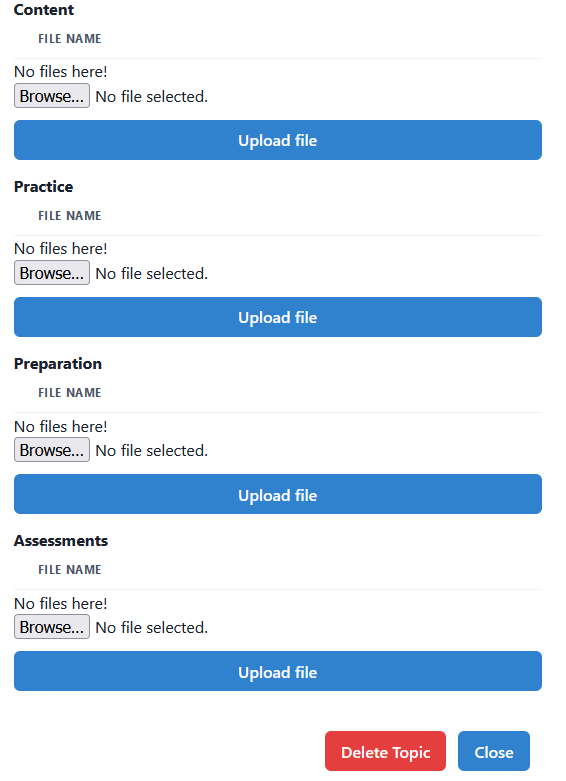
\includegraphics[scale=0.4]{topic-tree-file-sections}
    \caption{Topic Tree - File Sections}
\end{figure}

Users can also add a topic to a topic group, and add prerequisites to this topic in the same popup window. 

\begin{figure}[h!]
    \centering
    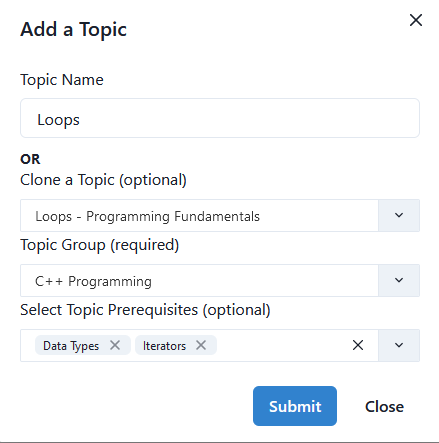
\includegraphics[scale=0.4]{topic-tree-add-topic-modal}
    \caption{Topic Tree - Add Topic}
\end{figure}

Users can also clone a topic i.e. if there is a topic in another topic group, academics can clone the materials in that topic and put it into another topic group. \\

Academics can also add topic groups, and search for a topic in the search bar in the header. Tags can be assigned to a topic which users can search for in the search bar to improve searchability of topics.

\begin{figure}[h!]
    \centering
    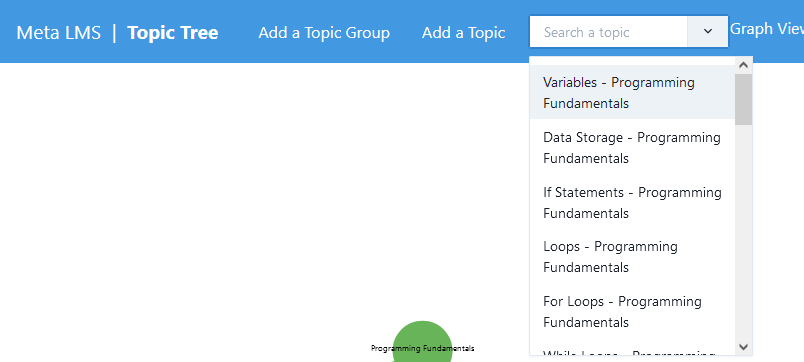
\includegraphics[scale=0.4]{topic-tree-search}
    \caption{Topic Tree - Search Bar}
\end{figure}
